\documentclass[
  bibliography=totoc,     % Literatur im Inhaltsverzeichnis
  captions=tableheading,  % Tabellenüberschriften
  titlepage=firstiscover, % Titelseite ist Deckblatt
  parskip=half, % !!! halbzeiliger vertikaler Abstand (siehe Latex-Skript S.125)
]{scrartcl}

% !!! Python in Latex
\usepackage{pythontex}

% !!! zum Drehen von Seiten
\usepackage{adjustbox}

% Paket float verbessern
\usepackage{scrhack}

% Warnung, falls nochmal kompiliert werden muss
\usepackage[aux]{rerunfilecheck}

% unverzichtbare Mathe-Befehle
\usepackage{amsmath}
% viele Mathe-Symbole
\usepackage{amssymb}
% Erweiterungen für amsmath
\usepackage{mathtools}

% Fonteinstellungen
\usepackage{fontspec}
% Latin Modern Fonts werden automatisch geladen
% Alternativ zum Beispiel:
%\setromanfont{Libertinus Serif}
%\setsansfont{Libertinus Sans}
%\setmonofont{Libertinus Mono}

% Wenn man andere Schriftarten gesetzt hat,
% sollte man das Seiten-Layout neu berechnen lassen
\recalctypearea{}

% deutsche Spracheinstellungen
\usepackage[ngerman]{babel}

% !!! babel mit anderen Sprachen laden für \enquote (siehe latex-Skript S.33)
\usepackage[autostyle]{csquotes}

% !!! zum durchstreichen durch \cancel{}
\usepackage{amsmath}
\usepackage[makeroom]{cancel}

% !!! zum Ersetzen von \symup{} durch z.B. \dif{}, siehe latex-Skript
\usepackage{expl3}
\usepackage{xparse}
\ExplSyntaxOn
\NewDocumentCommand \dif {m} {
  \mathinner{\symup{d} #1}
}
\ExplSyntaxOff

% !!! Nummerierung von Gleichungen nach Sections: Bei langen Dokumenten empfohlen (Chiristan)
% \usepackage{amsmath}
% \numberwithin{equation}{section}

% % !!! for den "token not defined in pdf"-Fehler, wenn man latex in \section{...} verwendet
% \PassOptionsToPackage{unicode}{hyperref}
% \PassOptionsToPackage{naturalnames}{hyperref} klappt nicht??


\usepackage[
  math-style=ISO,    % ┐
  bold-style=ISO,    % │
  sans-style=italic, % │ ISO-Standard folgen
  nabla=upright,     % │
  partial=upright,   % ┘
  warnings-off={           % ┐
    mathtools-colon,       % │ unnötige Warnungen ausschalten
    mathtools-overbracket, % │
  },                       % ┘
]{unicode-math}

% traditionelle Fonts für Mathematik
\setmathfont{Latin Modern Math}
% Alternativ zum Beispiel:
%\setmathfont{Libertinus Math}

\setmathfont{XITS Math}[range={scr, bfscr}]
\setmathfont{XITS Math}[range={cal, bfcal}, StylisticSet=1]

% Zahlen und Einheiten
\usepackage[
  locale=DE,                   % deutsche Einstellungen
  separate-uncertainty=true,   % immer Unsicherheit mit \pm
  per-mode=symbol-or-fraction, % / in inline math, fraction in display math
]{siunitx}

% chemische Formeln
\usepackage[
  version=4,
  math-greek=default, % ┐ mit unicode-math zusammenarbeiten
  text-greek=default, % ┘
]{mhchem}

% richtige Anführungszeichen
\usepackage[autostyle]{csquotes}

% schöne Brüche im Text
\usepackage{xfrac}

% Standardplatzierung für Floats einstellen
\usepackage{float}
\floatplacement{figure}{htbp}
\floatplacement{table}{htbp}

% Floats innerhalb einer Section halten
\usepackage[
  section, % Floats innerhalb der Section halten
  below,   % unterhalb der Section aber auf der selben Seite ist ok
]{placeins}

% Seite drehen für breite Tabellen: landscape Umgebung
\usepackage{pdflscape}

% Captions schöner machen.
\usepackage[
  labelfont=bf,        % Tabelle x: Abbildung y: ist jetzt fett
  font=small,          % Schrift etwas kleiner als Dokument
  width=0.9\textwidth, % maximale Breite einer Caption schmaler
]{caption}

% subfigure, subtable, subref
\usepackage{subcaption}

% Grafiken können eingebunden werden !!! von Jonas
\usepackage{graphicx}
%\usepackage{wrapfig}%Textumflossene Graphik
\usepackage{cancel} %Brüche Kürzen
\usepackage{tikz} %Fancy Kreisnummern
\usepackage[a4paper, left=30mm, top=30mm, right=30mm, bottom=40mm]{geometry} %Pagelayout
%\usepackage{subcaption} %Unterüberschrift
%\captionsetup[figure]{calcwidth=.85\linewidth} %You dont want to know
\usepackage{tasks} % Aufgaben

% !!! Für das Einfügen von pdfs wie messdaten etc.
\usepackage{pdfpages}

% schöne Tabellen
\usepackage{booktabs}

% Verbesserungen am Schriftbild
\usepackage{microtype}

% Literaturverzeichnis
\usepackage[
  backend=biber,
]{biblatex}
% Quellendatenbank
\addbibresource{lit.bib}
\addbibresource{programme.bib}

% Hyperlinks im Dokument
\usepackage[
  german,
  unicode,        % Unicode in PDF-Attributen erlauben
  pdfusetitle,    % Titel, Autoren und Datum als PDF-Attribute
  pdfcreator={},  % ┐ PDF-Attribute säubern
  pdfproducer={}, % ┘
]{hyperref}
% erweiterte Bookmarks im PDF
\usepackage{bookmark}

% Hinzugefügt
\usepackage{wrapfig}

% Trennung von Wörtern mit Strichen
\usepackage[shortcuts]{extdash}

% % !!! Seitenlayout (Jonas)
% \usepackage[headsepline=1pt,footsepline=1pt]{scrlayer-scrpage}
% \pagestyle{scrheadings}
% \clearpairofpagestyles

\author{%
  Toby Teasdale\\%
  \href{mailto:toby.teasdale@tu-dortmund.de}{toby.teasdale@tu-dortmund.de}%
  \and%
  Erich Wagner\\%
  \href{mailto:erich.wagner@tu-dortmund.de}{erich.wagner@tu-dortmund.de}%
}
\publishers{TU Dortmund – Fakultät Physik}
\setlength\parindent{0pt}

\subject{V64}
\title{Interferometrie}
\date{
  Durchführung: 12.04.23
  \hspace{3em}
  Abgabe: 14.04.23
}

\begin{document}

\maketitle
\thispagestyle{empty}
\tableofcontents
\newpage

\section{Ziel}
\label{sec:Ziel}
Das Ziel des Versuchs \enquote{He-Ne Laser} besteht darin, die Funktionsweise eine He-Ne Lasers kennenzulernen.
Außerdem wird sich mit der Justage beschäftigt und die Eigenschaften des Lasers vermessen, also die Wellenlänge, Intensitätsverteilung, Polarisation und Modenspektrum.
Zusätzlich werden verschiedene Einflüsse auf die Stabilität des Lasers getestet.
\section{Theorie}
\label{sec:Theorie}

Myonen sind instabile Elementarteilchen der Gruppe der Leptonen. 
Sie tragen ein negative Ladung, sind etwa 200-mal schwerer als Elektronen 
und haben eine Lebensdauer von ca. \qty{2,2}{\micro\second}.
Sie entstehen durch die Wechselwirkung hochenergetischer kosmischer Strahlung
mit den oberen Schichten der Atmosphäre,
auch bekannt als sekundäre kosmische Strahlung.
Aus Protonenschauern gehen Pionen hervor,
die über die Zerfälle
\begin{equation*}
    \pi^{+} \rightarrow \mu^{+}+\nu_\mu \qquad \text {und} \qquad \pi^{-} \rightarrow \mu^{-}+\bar{\nu}_\mu
\end{equation*}
schließlich Myonen erzeugen.
Die Lebensdauer eines instabilen Teilchens wird durch die Anzahl der Zerfälle pro Sekunde 
und pro Teilchen bestimmt, mit der es zerfällt. 
Sie folgt dem Zerfallsgesetz
\begin{equation} \label{eq:zerfallsgesetz}
    N(t) = N_0 \cdot \mathrm{e}^{-\lambda t} + U \, ,
\end{equation}
wobei $N_0$ die Anzahl der Anfangsteilchen, $\lambda$ die Zerfallskonstante
und $U$ Anzahl der Ereignisse der Untergrundstrahlung ist.
Diese berrücksichtigt die Umgebungsradioaktivität und kosmischer Strahlung.
Dabei stellt der Erwartungswert von $t$ die Lebensdauer $\tau$ dar und ergibt
\begin{equation} \label{eq:tau}
    \langle t\rangle=\tau=\int_0^{\infty} \lambda t \, \mathrm{e}^{-\lambda t} \mathrm{~d} t=\frac{1}{\lambda} .
\end{equation}

Klassisch haben Myonen nach Eintreten der Atmosphäre eine kurze Reichweite.
Da sie sich jedoch mit relativistischen Geschwindigkeiten bewegen,
bestizen sie aufgrund von Längenkontraktion eine deutlich größere Reichweite,
weswegen sie auch auf Meereshöhe mit einer Ereignisrate von $1 \, / \, 60\text{s} \, \text{cm}^2$ \cite[208]{grupen} messbar sind.


Um die in \autoref{eq:zerfallsgesetz} stehende Modifikation der Untergrundrate $U$ anzunähern,
wird ein Untergrundsignal als das Auftreffen einen Myons auf auf zweites angenommen,
was keinen Zerfall zur Folge hat.
Unter der weiteren Annahmne, 
dass die Wahrscheinlichkeit für dieses Ereignis poissonverteilt, 
ergibt sich die Anzahl der detektieren Myonen $n$ innerhalb der Suchzeit $T_\text{Such}$ zu
\begin{equation*}
    n=\frac{N_{0}}{T_{\text{Messung}}} \, ,
\end{equation*}
wobei $N_0$ die Anzahl der Startsignale und $T_{\text{Messung}}$ die Messzeit ist.
Mit dem Erwartungswert der gemessenen Ereignisse $T_\text{Such} \cdot n$ ergibt sich die Poissionverteilung zu
\begin{equation*}
    P(k)=\frac{\left(T_{\mathrm{Such}} \cdot n\right)^k}{k !} e^{T_{ \mathrm{Such}} \cdot n} \, .
\end{equation*}
Mithilfe der Wahrscheinlichkeit für ein weiteres Ereignis $P(1)$, 
kann die Anzahl der Fehlmessungen zu
\begin{equation*}
    N_{\mathrm{Fehl}}=N_{\mathrm{start}} \cdot P(1)
\end{equation*}
abgeschätzt werden.
Somit ergibt sich für ein Messkanal $N_\text{Kanal}$ die Untergrundrate
\begin{equation}\label{eq:untergrundrate}
    U=\frac{N_{\text {Fehl }}}{N_{\text {Kanal }}} \, .
\end{equation}


\subsection{Bauteile}
\label{sec:Bauteile}

In dem Folgenden werden die bei dem Versuch verwendeten Komponenten in ihrer prinzipiellen Funktionsweise erläutert.
\autoref{fig:schaltung} zeigt die Schaltung und die Bauteile.
\begin{figure}
    \centering
    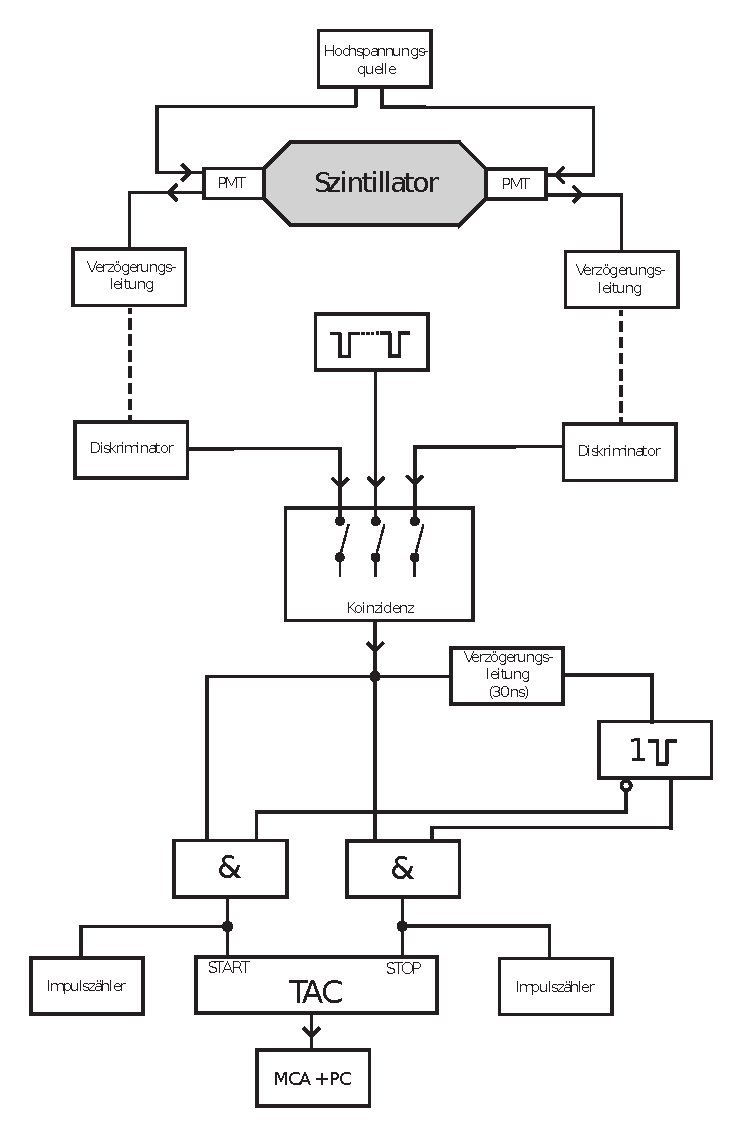
\includegraphics[width=0.8\textwidth]{pictures/schaltung.pdf}
    \caption{Blockschaltbild des Versuchsaufbaus \cite[3]{v01}.}
    \label{fig:schaltung}
\end{figure}


\subsubsection*{Photomultiplier}
Ein Photomultiplier (PMT) ist ein Detektor, der in der Teilchenphysik, 
der Astronomie und anderen Bereichen eingesetzt wird, um einzelne Photonen zu erfassen und zu verstärken. 
Bei der Messung der Lebensdauer kosmischer Myonen wird ein Photomultiplier (PMT) verwendet, 
um das Lichtsignal zu registrieren, das entsteht, 
wenn ein Myon in einem Szintillationsdetektor zerfällt. 

\subsubsection*{Szintillationsdetektor}
Ein Szintillator ist ein Detektor, der in der Lage ist, 
ionisierende Strahlung wie beispielsweise kosmische Strahlung zu detektieren. 

Es gibt verschiedene Arten von Szintillatoren wie organische und anorganische Szintillatoren,
die sich in ihrer Funktionsweise und ihrem Anwendungsgebiet unterscheiden.

Organische Szintillatoren bestehen aus einem organischen Material.
Die darin eindringenden Teilchen regen die Moleküle des Materials zu Schwingungen an. 
Nach Abgabe eines Photons gehen die angeregten Moleküle wieder in den Grundzustand über.
Der Vorteil dieses Material besteht deswegen in der Zeitauflösung, 
während eine Energieauflösung aufgrund der breiten Frequenzmodenverteilung benachteiligt ist.

Anorganische Szintillatoren bestehen aus anorganischen Materialien wie Kristallen oder Keramik. 
Dabei ionisiert sich das Material und erzeugt nach Aktivierung ein Lichtsignal.
Anders als beim organischen Material, liegen hier diskrete Ionisationsenerigen vor,
weswegen eine höhere Energieauflösung möglich ist.

\subsubsection*{Verzögerungsleitung}
Die Verzögerungsleitungen gleichen Unterschiede in der Signalübermittlung aus
und werden hier anpassbare bzw. zuschaltbare Kabel realisiert.

\subsubsection*{Diskriminator}
Das durch die Verzögerungsleitung gehende Signal wird durch Diskriminatoren geleitet.
Dabei wird das schwankende Signale der Photomultiplier ab einer gewissen Schwelle in diskrete
Ereignissignale umwandelt.

\subsubsection*{Koinzidenz}
Anschließend erreichen beide Signale eine Koinzidenzschaltung, welche ein Ausgangssignal
erzeugt, sobald zwei Photomultiplier gleichzeitig ein Signal aussenden.

\subsection*{Univibrator}
Der Univibrator, oder auch Monoflop bzw. monostabile Kippstufe genannt,
bleibt nach Eingang eines Signal nur für eine voreingestellte Zeit eingeschaltet.

\subsection*{Time-Amplitude-Converter}
Nachdem die Signale die AND-Gatter passieren, 
gelangen sie zeitversetzt zum Time-Amplitude-Converter (TAC).
Das Ausgangssignal des TACs ist hierbei proportional zur Zeitdifferenz der beiden Signale.

\subsection*{Multi-Channel-Analyzer}
Der Multi-Channel-Analyzer (MCA) oder Vielkanalanalysator ordnet die eingehenden Signale
abhängig von ihrer Amplitude als Histogramm in Kanälen an.
Im Rahmen dieses Versuchs wird die Energie der Myonen gegen die Anzahl der Ereignisse aufgetragen. 
Die erwartete Verteilung sollte eine charakteristische exponentielle Abnahme der Ereignisanzahl mit 
zunehmender Energie aufgrund des exponentiellen Zerfalls der Myonen zeigen.
\section{Durchführung}
\label{sec:Durchführung}

In dem hier vorhandenen Aufbau liegt ein \enquote{D8-Labordiffraktometer} der Firma Bruker-AXS vor.
Dabei entsteht die Röntgenstrahlung gemäß \autoref{sec:Röntgenstrahlung} in einer Kupferanodenröhre, die mit einem Strom von $I=35\unit{\milli\ampere}$ 
und einer Spannung von $U = 40 \unit{\kilo\volt}$ betrieben wird.
Der Strahl wird mithilfe eines Göbelspiegels gebündelt und monochromatisiert.
Die Wellenlänge des Röntgenstrahls beträgt dann $\lambda = 1,55 \unit{\angstrom}$, da es sich um die $K_\alpha$-Linie von Kupfer handelt.

\subsection{Justage} \label{sec:Justage}

Bei der Justage kommen insgesamt vier verschiedene Arten von Scans zum Einsatz.
Begonnen wird dabei mit dem \textbf{Detektorscan}.
Diese Messung dient dazu, die Nulllage des Detektors zu finden und damit die Intensität des Strahles zu maximieren.
Die Probe wird aus dem Strahlengang entfernt, damit der Strahl ungehindert durch den Raum propagieren kann.
Dann wird die Position gesucht, in der die Intensität des Strahles maximal ist und als neue Nulllage definiert.

Im Anschluss wird ein sogenannter \textbf{Z-Scan} durchgeführt.
Wie der Name bereits andeutet, handelt es sich um einen Scan zur Justage der z-Achse.
Dafür wird zunächst die Probe wieder in den Strahlengang geschoben.
Die z-Position der Probe wird so lange variiert, bis die Intensität mit Probe auf die halbe Intensität ohne Probe abgesunken ist, also $I_{z,\text{Probe}} = \frac{I_\text{max}}{2}$.
Auf dieser $z$ Position wird dann der Probentisch gehalten.

Nun wird ein \textbf{X-Scan} durchgeführt.
Dabei wird der Probentisch senkrecht zum Strahl (x-Achse) bewegt.
Hierbei wird überprüft, das der Strahl auch wirklich die Probe und nicht den Tisch trifft.
Dies wird dadurch getestet, dass die Intensität des Strahls abnimmt, während er durch die Probe abgeschirmt wird.
Im Anschluss wird eine beliebige Position in diesem Minimum gewählt.   

Nun wird zu dem \textbf{Rockingscan} übergegangen.
Dabei handelt es sich um einen Scan, bei dem die Röhre und Detektor in einer festen Achse um die Probe rotiert werden.
Durch diesen Scan kann eine Mögliche Verkippung der Probe detektiert werden.
Außerdem kann durch ihn die Probe (durch mögliche Fehlpositionierung auf dem Tisch) in den Drehpunkt des Diffraktometers gebracht werden.
Zwischen Detektor und Probe wird dabei ein Winkel von $2 \Theta = 0$ beibehalten.
Die Messung wird durch kleine Schritte im Bereich $[-1°,1°]$ durchgeführt.
ist das Maximum in der Intensität gefunden, wird der entsprechende Winkel notiert.

Nun kommt es zur Feinjustage der Probe.
Dabei wird zunächst ein Z-Scan und dann zwei weiterere Rockingscans (bei $2 \Theta = 0,3°$ und $2 \Theta = 0,5°$) durchgeführt.
Nun kann zur eigentlichen Messung übergegangen werden.

\subsection{Tatsächliche Messung}
Für die tatsächliche Messung wird der Winkel des Detektors und der Röhre auf null gestellt und $2 \Theta$ ebenfalls.
Dann wird unter dem Modus \enquote{Omega/2Theta} im Bereich $[0 \, , \, 2,5]$ eine Messung mit einer Zeit pro Messwert von $5 \unit\second$ aufgenommen.
Nun kann das Messprogramm gestartet werden.
Im Anschluss daran wird noch eine \enquote{Diffuse}-Messung durchgeführt.
Dafür wird der Winkel des Detektors auf $0,1°$ gestellt.
Der Rest wird analog zur Messung davor eingestellt und das Messprogramm kann gestartet werden.
+\section{Fehlerrechnung}
\label{sec:Fehlerrechnung}

Im Folgenden wird die allgemeine Fehlerrechnung und alle wichtigen Größen der entsprechenden Rechnung erklärt.
Die wichtigsten Werte dabei sind der 
\begin{align}
    \text{Mittelwert} \quad & \bar{x}  = \frac{1}{N} \sum_{i=0}^{n} x_i \quad \text{und die} \label{eq:mittelwert} \\
    \text{Standartabweichung} \quad & \sigma  = \sqrt{\frac{1}{N - 1 } \sum_{i=0}^{N} (x_i -  \bar{x})^2} \, . \label{eq:standartabweichung}
\end{align}

Dabei entspricht $N$ der Anzahl an Werten und $x_i$ ist jeweils ein mit einem Fehler gemessener Wert.
Es ergibt sich ebenfalls die statistische Messunsicherheit
\begin{equation}
    \increment \bar{x} = \frac{\sigma}{\sqrt{N}} = 
    \sqrt{\frac{1}{N(N - 1)} \sum_{i=0}^{N} (x_i -  \bar{x})^2} \, . \label{eq:messunsicherheit}
\end{equation} 

Entstehen mehrere Unbekannte in einer Messung, folgen daraus auch mehrere Messunischerheiten,
die in dem weiteren Verlauf der Rechnung berücksichtigt werden müssen.
Es gilt die \textit{Gaußsche Fehlerfortplanzung}
\begin{equation}
    \increment f(y_1 ,y_2 ,...,y_N ) = \sqrt{\left(\frac{\dif{f}}{\dif{y_{1}}} \increment y_{1}\right)^2
    + \left(\frac{\dif{f}}{\dif{y_{2}}} \increment y_{2}\right)^2 + ... + 
    \left(\frac{\dif{f}}{\dif{y_{N}}} \increment y_{N}\right)^2
    } \, . \label{eq:fehlerfortplanzung}
\end{equation}
\section{Auswertung}
\label{sec:Auswertung}

Im folgenden werden die Daten analysiert, die während einer Messzeit von ungefähr $T_\text{Messung} = 4,7  \, \unit\day$ aufgenommen wurden.
Die Plots und Fits sind alle mit den Python-Bibliotheken \cite{matplotlib},\cite{numpy},\cite{scipy},\cite{uncertainties},\cite{reback2020pandas} erstellt worden.
\subsection{Kalibrierung der Messgeräte}

Bei der Kalibrierung der Geräte trat ein Problem bei der Einstellung der Pulsdauer auf.
Aus diesem Grund wurde die Pulsdauer statt auf $10 \, \unit{\nano\second}$ und $20 \, \unit{\nano\second}$ auf $20 \, \unit{\nano\second}$ und $30 \, \unit{\nano\second}$ eingestellt.
Die Messdaten dazu sind im Anhang in \autoref{tab:20ns_table} und \autoref{tab:30ns_table} zu finden.
Die Plots der Daten und der entsprechenden Halbwertsbreiten sind in \autoref{fig:20ns_plot} und \autoref{fig:30ns_plot} abgebildet.
Auch bei der Aufnahme der Daten kam es zu Problemen, siehe dafür \autoref{sec:Diskussion}.
Hier sei allerdings angemerkt, dass die Halbwertsbreiten deshalb nur abgeschätzt werden können.
Nun soll aus dieser Abschätzung die optimale Verzögerung ermittelt werden.
Hierfür wird die Formel
\begin{equation*}
    t_\text{Verzögerung} = 2 \cdot \Delta_\text{Pulsdauer} - \Delta_\text{Breite}
\end{equation*}
genutzt. Sie berechnet die Verschiebung des Maximums und liefert somit die optimale Verzögerungszeit.
Für eine Pulsdauer von $20 \, \unit{\nano\second}$ ergibt sich eine Halbwertsbreite von $\Delta_\text{Breite} = 25 \, \unit{\nano\second}$, woraus sich dann eine Verzögerung von
\begin{equation*}
    t_\text{Verzögerung} = (2 \cdot 20 - 25) \, \unit{\nano\second} = 15 \, \unit{\nano\second}
\end{equation*}
ergibt.
Für eine Pulsdauer von $30 \, \unit{\nano\second}$ ergibt sich eine Halbwertsbreite von $\Delta_\text{Breite} = 37 \, \unit{\nano\second}$, woraus sich dann eine Verzögerung von
\begin{equation*}
    t_\text{Verzögerung} = (2 \cdot 30 - 37) \, \unit{\nano\second} = 23 \, \unit{\nano\second}
\end{equation*}
ergibt.

\begin{figure}
    \centering
    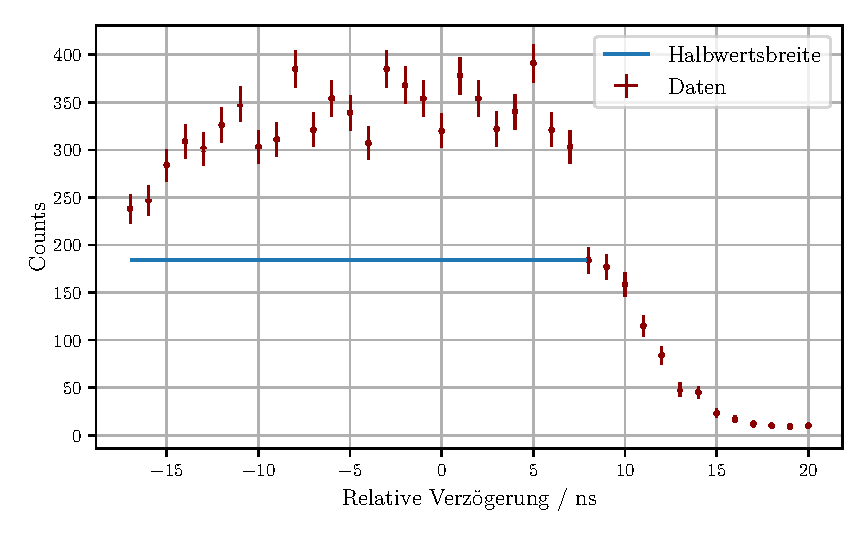
\includegraphics[width = 0.7 \linewidth]{build/20ns_plot.pdf}
    \caption{Plot der Messung der Zählrate in Abhängigkeit der relativen Verzögerung bei einer Pulsdauer von $20$ ns.}
    \label{fig:20ns_plot}
\end{figure}

\begin{figure}
    \centering
    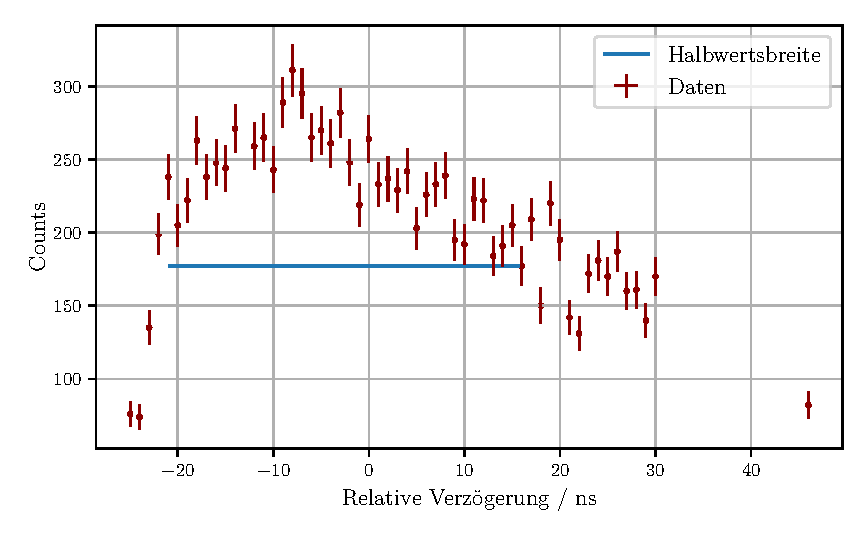
\includegraphics[width = 0.7 \linewidth]{build/30ns_plot.pdf}
    \caption{Plot der Messung der Zählrate in Abhängigkeit der relativen Verzögerung bei einer Pulsdauer von $30$ ns.}
    \label{fig:30ns_plot}
\end{figure}

\subsection{Bestimmung der Zeiteinteilung der Bins am TCA} \label{sec:zeiteinteilung}

Die Messdaten sind in \autoref{tab:zeiteinteilung} zu finden.
Um den Bins des TCAs eine Zeit zuzuordnen, wird eine Regressionsrechnung durchgeführt.
Dafür wird der Ansatz
\begin{equation*}
    t = m \cdot b + c
\end{equation*}
gewählt.
Der entsprechende Plot ist in \autoref{fig:zeiteinteilung} abgebildet.
Der Fit ergibt 
$m = (0.02257 \pm 0.00005) \, \unit{\micro\second}$ und $c = (0.148 \pm 0.006) \, \unit{\micro\second}$.


\begin{figure}%
    \begin{subfigure}{0.68\textwidth}%
    \centering%
    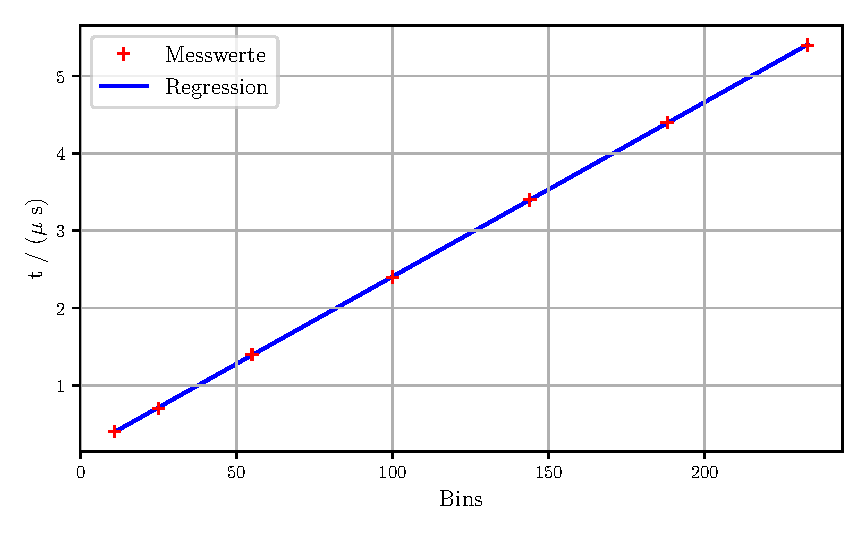
\includegraphics[width=\textwidth]{build/zeiteinteilung.pdf}%
    \caption{Abbildung der Messdaten zur Bestimmung der Zeiteinteilung der Kanäle. Die Gerade zeigt den linearen Fit zur Zuordnung der Kanäle.}%
    \label{fig:zeiteinteilung}%
    \end{subfigure}%
    \hfill% Fills available space in the center -> space between figures
    \begin{subtable}{0.28\textwidth}%
        \centering
        \begin{tabular}{c c}
        \toprule
        t / $(\unit{\micro\second})$ &  Bins \\
        \midrule
         5.4 & 233 \\
         4.4 & 188 \\
         3.4 & 144 \\
         2.4 & 100 \\
         1.4 &  55 \\
         0.7 &  25 \\
         0.4 &  11 \\
        \bottomrule
        \end{tabular}
        \caption{Messdaten zur Bestimmung der Zeiteinteilung der Kanäle.}
        \label{tab:zeiteinteilung}
    \end{subtable}%
    \caption{Bestimmung der Zeiteinteilung der Bins.}
    \label{subfig:zeiteinteilung}    
\end{figure}%
    
\subsection{Bestimmung der Lebenszeit von Myonen}

\begin{figure}%
    \begin{subfigure}{0.5\textwidth}%
    \centering%
    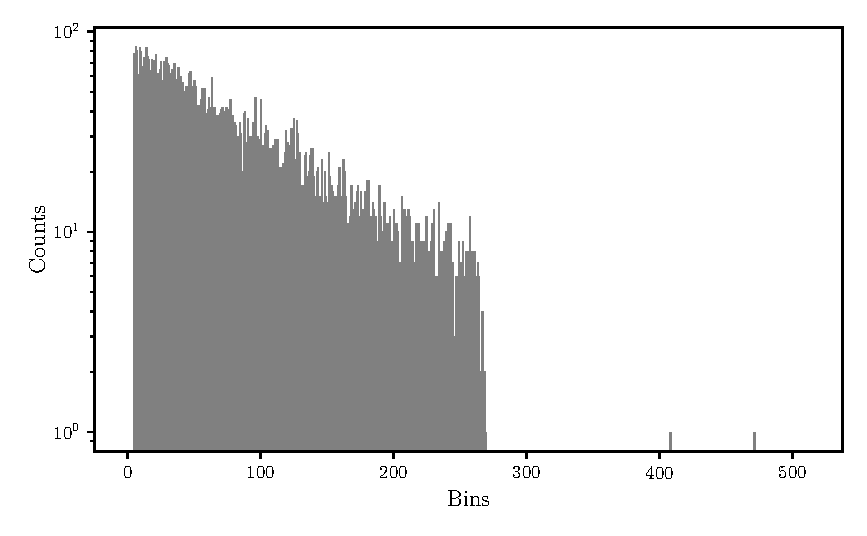
\includegraphics[width=\textwidth]{build/myonenhist.pdf}%
    \caption{Histogramm der Messdaten.}%
    \label{fig:histogramm}%
    \end{subfigure}%
    \hfill% Fills available space in the center -> space between figures
    \begin{subfigure}{0.5\textwidth}%
        \centering%
        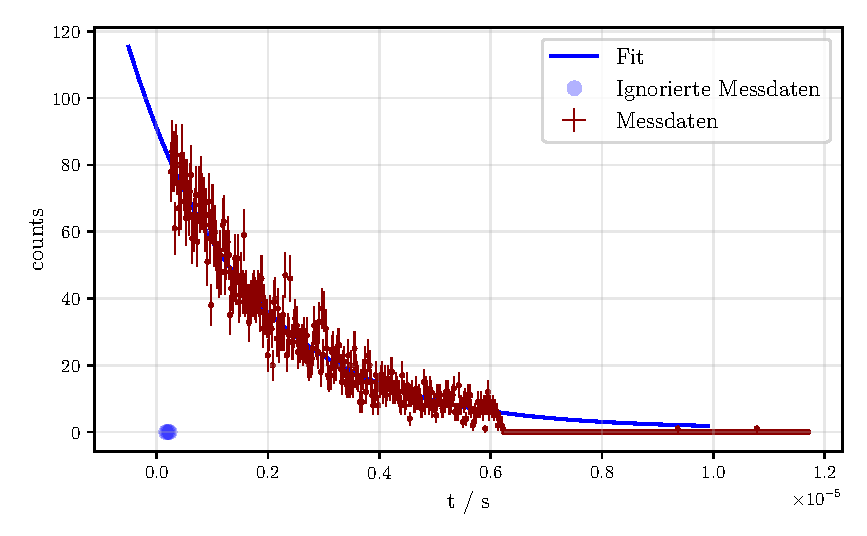
\includegraphics[width=\textwidth]{build/myonenfit.pdf}%
        \caption{Das Resultat des Fits an die Messdaten}%
        \label{fig:myonenfit}%
        \end{subfigure}%
    \caption{Abbildungen zur Ermittlung der Lebenszeit eines Myons.
    Links sind die Messwerte histogrammiert auf einer logarithmischen Skala abgebildet.
    Rechts ist der entsprechende Fit abgebildet.}
    \label{subfig:myonen}    
\end{figure}%

Die Messdaten zu diesem Versuch sind im Anhang in \autoref{tab:messdaten_myonen1}, \autoref{tab:messdaten_myonen2} und \autoref{tab:messdaten_myonen3} zu finden.
Die Daten wurden außerdem histogrammiert in \autoref{fig:histogramm} aufgetragen.
Die gezählten Ereignisse und Ereignisse, die verworfen wurden, sind in \autoref{fig:myonenfit} abgebildet.
Dabei muss beachtet werden, dass der Counter, der die Events zählt, einmal durchgelaufen ist.
Als Fit wird nach Vorgabe des Zerfallsgesetzes plus Untergrund die Funktion
\begin{equation*}
    N(t) = N_0 \cdot e^{- \lambda t} + U
\end{equation*} 
angesetzt.
Dabei wird stets beachtet, dass die Konstanten größer null sein müssen.
Außerdem werden die ersten vier Bins nicht beachtet, da diese mit null gefüllt sind.
Dies liegt an der vorgeschalteten Verzögerung, somit kann hier kein Ereignis gezählt werden.
Der Fit ergibt $N_0 = 92.5 \pm 1.0$, $\lambda = (4.78 \pm 0.10) \cdot 10^5 \frac{1}{\unit{\second}}$ und $U = 0.00 \pm 0.31$.
Es gilt $U \in [0 \, , \, 0,31]$, da der Untergrund stets positiv ist.
Der entsprechende Plot ist in \autoref{fig:myonenfit} abgebildet.
Hier wurde auch bereits mit der Formel für die Zeit aus \autoref{sec:zeiteinteilung} dem jeweiligen Bin eine Zeit zugeordnet.
Aus $\lambda$ lässt sich nun mithilfe \autoref{eq:tau} die Lebenszeit bestimmen.
Es ergibt sich
\begin{equation}
    \tau = \frac{1}{\lambda} = (2.09\pm 0.04) \, \unit{\micro\second} \, .
\end{equation}

\subsection{Bestimmung des Untergrundes} \label{sec:untergrund_ausw}

Nachdem bereits der Untergrund gefittet wurde, soll dieser auch nach der theoretischen Formel \autoref{eq:untergrundrate} berechnet werden.
Es ergibt sich mit
\begin{equation*}
    n = (26.092\pm0.008) \frac{1}{\unit\second}
\end{equation*}
und
\begin{equation*}
    P(1) = (2.6098 \pm 0.0008) \cdot 10^{-4}
\end{equation*}
der theoretische Untergrund von
\begin{equation*}
    U_\text{theo} = 5.4008 \pm 0.0033 \, .
\end{equation*}
\section{Diskussion}
\label{sec:Diskussion}

Die ermittelte horizontale Komponente des Erdmagnetfeldes von $B_\text{H} = \qty{23.9(5)}{\micro\tesla}$
weicht relativ gering von dem erwarteten Wert von etwa $\qty{20}{\micro\tesla}$ ab.
Das Vorjustieren der Messapparatur durch beispielsweise richtige Ausrichtung des Tisches oder
etwa das schmaler machen des ersten Peaks können dabei diese Abweichung bedingen.

Die bestimmten g-Faktoren liegen relativ nahe an den theoretischen Werten von
$g_{\text{F}_{85}}= 1/2$ und $g_{\text{F}_{87}}= 1/3$. 
Selbiges gilt für die berechneten Kernspins im Vergleich mit den theoretischen von
$I_{85}=3/2$ und $I_{87}=5/3$.
Auch hier bedingt größtenteils das Ablesen der Peaks die Abweichung.

Das abgeschätzte Isotopenverhältnis von $0.51$ entpsricht auch hier in etwa dem tatsächlichen Verhältnis.


\newpage
\printbibliography{}
\nocite{matplotlib}
\nocite{numpy}
\nocite{scipy}
\nocite{uncertainties}
\nocite{reback2020pandas}

\newpage
% 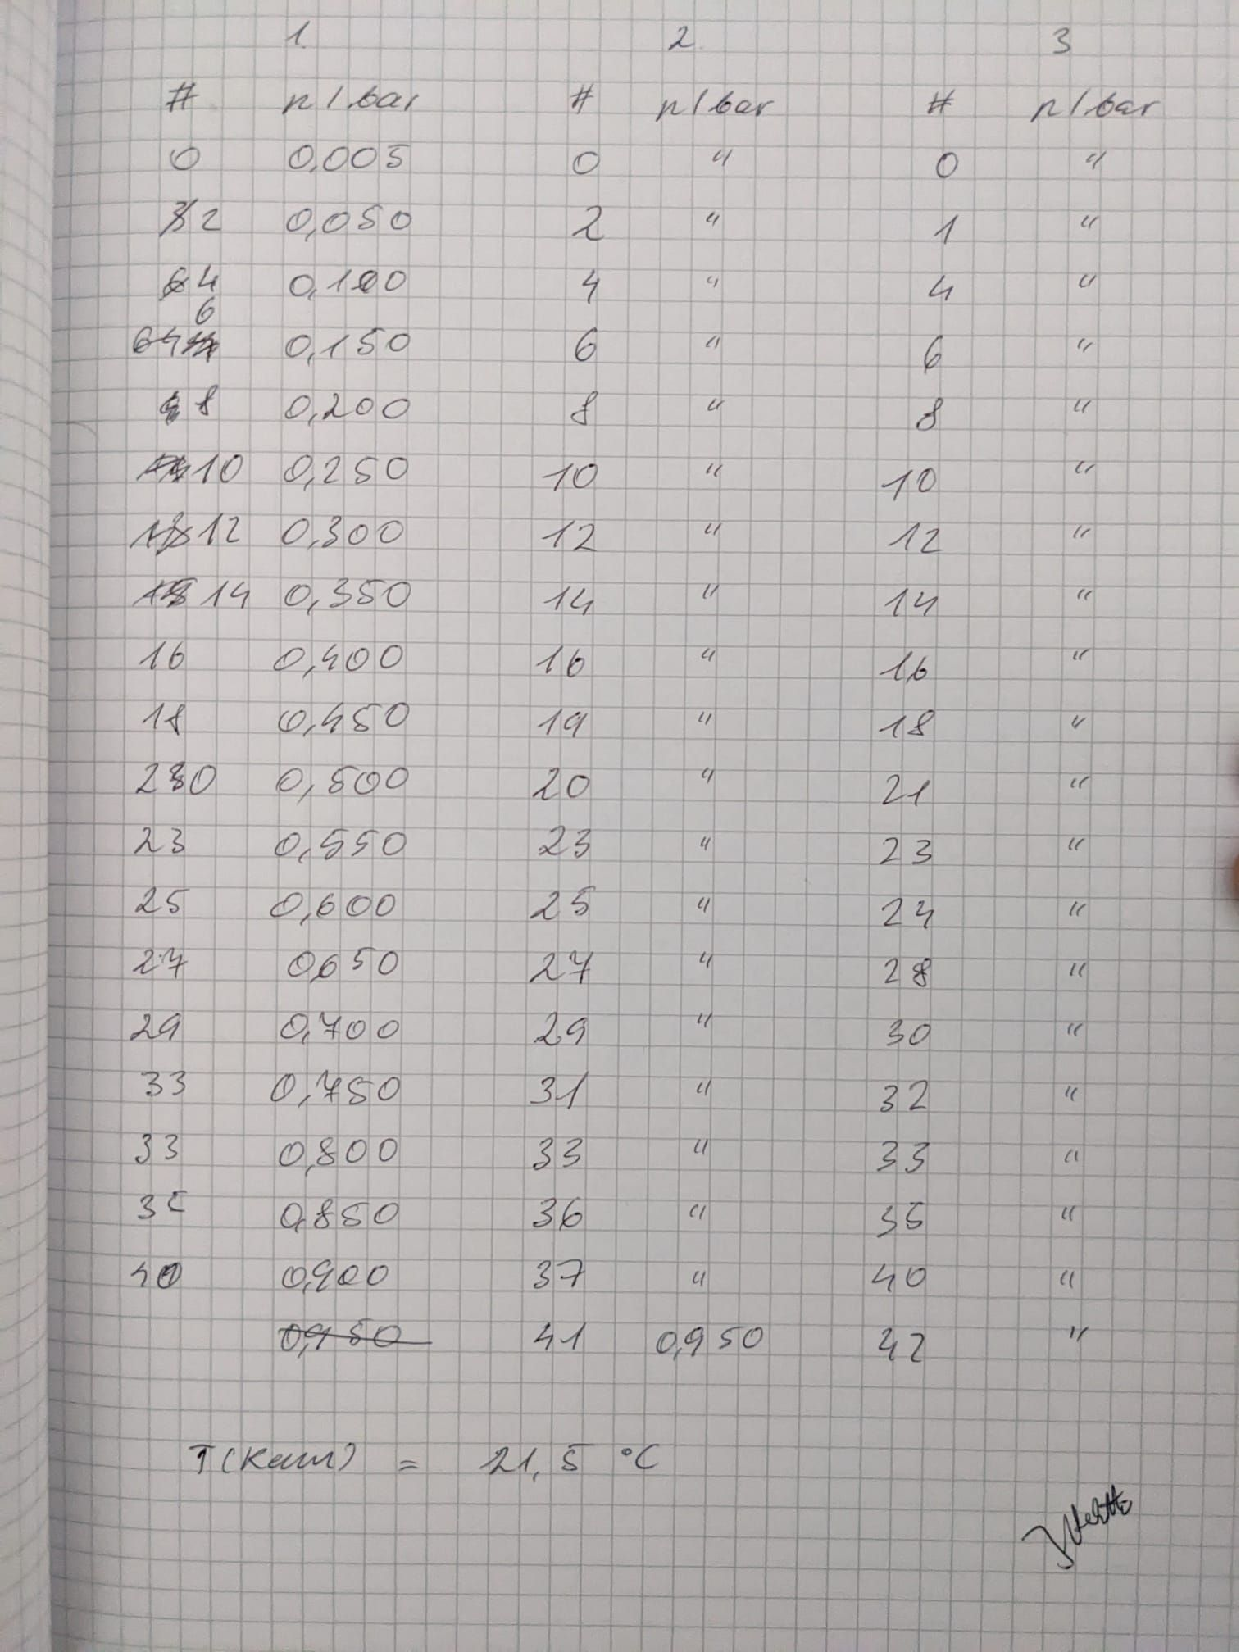
\includepdf[pages=-]{tables/messdaten.pdf}

\end{document}
